In the previous section we presented three WSN simulators commonly used.
\\
    Both NS-2 and J-Sim were not designed especially for wireless 
sensor network simulators but the basic applications were extended
in order to support WSN simulations; TOSSIM was especially designed
for the Berkeley Mica Mote platform and aims to simulate rather TinyOS's behavior
than general sensors. Even though they provide a good simulation environment,
we believe a simulator targeted for wireless sensors will offer better results
and take into consideration more of the particularities a WSN has.
\\
    Simulators are mainly used for research purposes, and if some tested solution
offers good results it is very likely that it will be eventually ported on 
read-world devices. The less effort needs to be invested in this porting, the
better. Of the three simulators presented, nesC TOSSIM code is the easiest to port,
but only on TinyOS motes, C/C++ NS-2 code can be ported as well but at a higher
cost whereas Java J-Sim's code cannot be ported but the solution should be 
reimplemented in a programming language that can be run on sensors.
\codename will be written in C with a declared purpose of being very easy to port
on real-world sensors.
\\
All three presented simulators lack detailed environment modeling: J-Sim has 
antenna component to model signal transmissions and TOSSIM provides a configuration
file to define the probability that a sent bit will be received corrupted. 
 none of them
being capable of 3D indoor simulation without modification. 
\\

\subsection{Architecture}
\begin{center}
	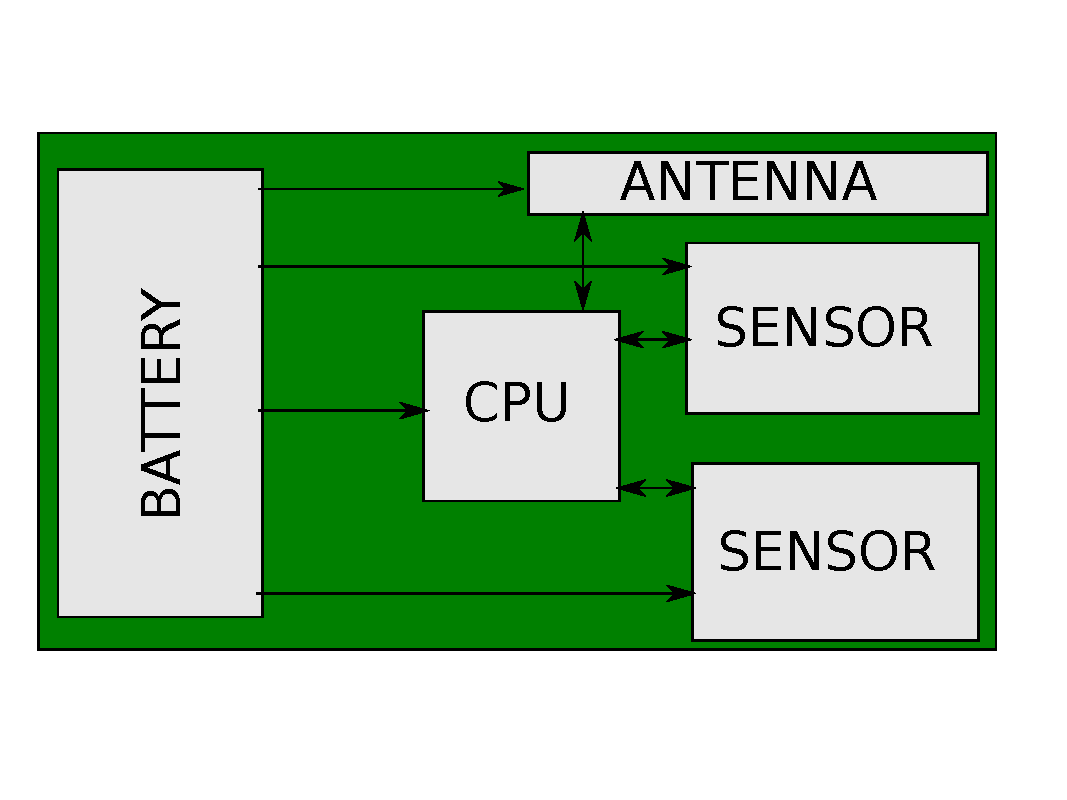
\includegraphics[scale=0.6]{img/board.pdf}
\end{center}
\label{subsec:architecture}

The simulator we will be building will have a modular design. Each type
of component, a battery or a sensor, will a have a template containing a
very basic implementation of it. For example a transceiver template will
have a template consisting of the send() and recv() methods, but more
usefull implementations will be built on this to take into account the
environment and power consumption. On top of this template many different
implementations may be derived; for example a lithium-ion battery or a solar
powered one. Each component will provide an access interface for other components
(a sensor might have a read_data() interface) and they will not depend on other 
components. This way we will be able to simulate a wide range of platforms by
combining different components in different slots.

All the activity on one node will be coordinated by a CPU component. This will provide
an API to the routing protocol running on the node for activities such as allocating memory 
and sending and receiving packets. To simulate a slower node, the code running on the 
node will be ran using the \textit{ptrace} system call. The protocol will set in the beginning
breakpoints at every point in the program and the parent process(the node) will limit
its speed based on a configured value. We do not see any reasons to have more than one
type of CPU so only one will be available, but its performance and available memory
will be configurable.

Data through the network will not come only from the routing protocol, but sensors on the 
node will be able to generate realistic data that will accurately model the normal load
on such a network. This is important in order to see how protocols behave under load 
because some of them work by aggregating data.

It is important to be able to gather information from the network(number of packets sent
or received, battery life, power consumption per device) so there will be a central agent
responsible for gathering this information. Each component will send the statistics gathered
by them to the agent who will be able to present them in a more usefull form (bars and pies).

\subsection{Components}
\subsection{Environment}
%\begin{center}
%	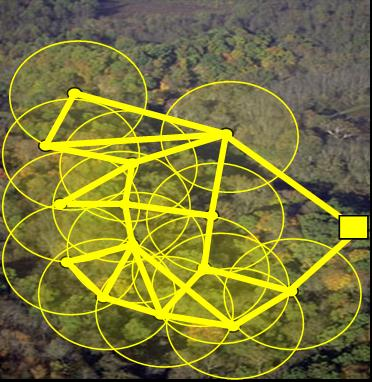
\includegraphics{img/env.jpg}
%\end{center}

\fig[scale=0.7]{img/env.jpg}{img:env}{Sensors and their area of signaling}
Wireless Sensor Networks are deployed in a wide range of environments. This affects
the way the routing protocols perform and the way hierarchies are formed. An indoor
environment for example means that the nodes will have to use more power to transmit
packets which will lead to lower battery life. We think it is important to be able to
see how this protocols behave in a real environment. This will be very important for
mobile nodes, which can change their location, as simple attenuation based design will
not be able to simulate realistically the effects of the environment on power needed for
transmisions. In an environment without atenuation 
the sensors' signals would look like shown in \figref{img:env}. 

The environment will
include nodes (for simulating nodes placed in a fixed way -useful when running the same
simulation more than once- the nodes can be placed directly in the environment) and data sources
(to simulate data for the networks, data sources will be placed in
the environment, when a node gets in contact with it, the sensor will generate data packets; 
they can be stationary, mobile or affect an area).

%\begin{itemize}
%	\item Nodes. For simulating nodes placed in a fixed way(useful when running the same
%simulation more than once) the nodes can be placed directly in the environment.
%	\item Data sources. To simulate data for the networks, data sources will be placed in
%the environment, when a node gets in contact with it, the sensor will generate data packets. 
%They can be stationary, mobile or affect an area.
%\end{itemize}

Environments will be designed in Blender, a 3D graphics tool, from which they will be
exported to our simulator using its extensive scripting support. They will be visible
in the GUI of \codename, along with the nodes.



